
\section{Bedienoberfläche}

%Hier sollen die Skizzen/Prototypen von Bedienoberflächen dargestellt werden, als auch die Zusammenhänge zwischen denen (wie gelingt man von einem zu dem anderen Fenster/Ansicht). Ein Beispiel für Bildereinbau in LaTeX ist die Abbildung~\ref{gui:zusammenhang}.\footnote{Bevor Sie mit den Skizzen anfangen, überlegen Sie sich, welche virtuelle Räume im System zu haben sind und dann halte Sie die Namen der GUI-Fenstern mit diesen konsistent.}

\newcounter{gui}\setcounter{gui}{10}

\begin{description}[leftmargin=5em, style=sameline]	
	\begin{lhp}{gui}{GUI}{gui:beispiel}
		\item[Name:] Vorraum-Interface.
		\item[Beschreibung:] Interface für die Wahl zwischen Anmeldung oder Registrierung.
		\item[Relevante Systemfunktionen:] \ref{funk:zugriff}
		\item[Abbildungen:] \ref{gui:willkommen}
	\end{lhp}
\end{description}
\begin{description}[leftmargin=5em, style=sameline]	
	\begin{lhp}{gui}{GUI}{gui:beispiel}
		\item[Name:] Einloggen-Interface.
		\item[Beschreibung:] Interface für die Anmeldung des Spielers.
		\item[Relevante Systemfunktionen:] \ref{funk:zugriff}
		\item[Abbildungen:] \ref{gui:login}
	\end{lhp}
\end{description}

\begin{description}[leftmargin=5em, style=sameline]	
	\begin{lhp}{gui}{GUI}{gui:beispiel}
		\item[Name:] Registrierung.
		\item[Beschreibung:] Interface für die Registrierung.
		\item[Relevante Systemfunktionen:] \ref{funk:zugriff}
		\item[Abbildungen:] \ref{gui:register}
	\end{lhp}
\end{description}
\begin{description}[leftmargin=5em, style=sameline]	
	\begin{lhp}{gui}{GUI}{gui:beispiel}
		\item[Name:] Anmeldungsfehler.
		\item[Beschreibung:] Hat der Spieler einen falschen Benutzername und/oder Passwort eingegeben, wird der Anmeldungsfehler angezeigt. Und der Spieler hat die Möglichkeit, sie nochmal einzugeben.
		\item[Relevante Systemfunktionen:] \ref{funk:zugriff}
		\item[Abbildungen:] \ref{gui:warning1}
	\end{lhp}
\end{description}
\begin{description}[leftmargin=5em, style=sameline]	
	\begin{lhp}{gui}{GUI}{gui:beispiel}
		\item[Name:] Registrierungsfehler.
		\item[Beschreibung:] Beim Registrieren kann es sein, dass der Spieler einen von anderem Spieler benutzten Benutzername eingibt. In diesem Fall wird einen Registrierungsfehler angezeigt.
		\item[Relevante Systemfunktionen:] \ref{funk:zugriff}
		\item[Abbildungen:] \ref{gui:warning2}
	\end{lhp}
\end{description}
\begin{description}[leftmargin=5em, style=sameline]	
	\begin{lhp}{gui}{GUI}{gui:beispiel}
		\item[Name:] Startseite.
		\item[Beschreibung:] Nach dem Einloggen ist die Startseite so dargestellt, dass der Spieler sein Profil, die Lobbies sowie das Chat$-$Fenster sehen kann. In der Startseite kann er einen Spielraum erstellen, sein Profil bearbeiten oder sich sogar ausloggen.
		\item[Relevante Systemfunktionen:] \ref{funk:zugriff} \ref{funk:chat}
		\item[Abbildungen:] \ref{gui:profil}
	\end{lhp}
\end{description}
\begin{description}[leftmargin=5em, style=sameline]	
	\begin{lhp}{gui}{GUI}{gui:beispiel}
		\item[Name:] Interface für die Bearbeitung eines Profils.
		\item[Beschreibung:] Das Interface bietet dem Spieler die Möglichkeit, seine Eingaben zu ändern; wie das Profilbild, den Spielername oder das Passwort. Er kann aber auch sein Profil löschen.
		\item[Relevante Systemfunktionen:] \ref{funk:zugriff}
		\item[Abbildungen:] \ref{gui:modifieprofil}
	\end{lhp}
\end{description}
\begin{description}[leftmargin=5em, style=sameline]	
	\begin{lhp}{gui}{GUI}{gui:beispiel}
		\item[Name:] Interface für die Erstellung einer neuen Lobby(Spielraum).
		\item[Beschreibung:] Hier kann der Spieler eine neue Lobby mit einem passenden Passwort erstellen. (Mit diesem Passwort können andere Spieler der Lobby beitreten.)
		\item[Relevante Systemfunktionen:] \ref{funk:spielraum}
		\item[Abbildungen:] \ref{gui:spielraumerstellen}
	\end{lhp}
\end{description}
\begin{description}[leftmargin=5em, style=sameline]	
	\begin{lhp}{gui}{GUI}{gui:beispiel}
		\item[Name:] Lobby-Interface.
		\item[Beschreibung:] In dem Lobby-Interface können die Spieler des Spielraumes nach Name oder gespielten Spielen oder gewonnenen Spielen geordnet (wie einer Bestenliste). Spieler sowie Bots können auch hinzugefügt oder entfernt werden. Zusätzlich ist das Chat$-$Fenster ein Teil des Interfaces. Sind alle Spieler bereit, können sie dann auf "LOS GEHT'S" klicken, und das Spiel startet.
		\item[Relevante Systemfunktionen:] \ref{funk:spielraum} \ref{funk:bestenliste} \ref{funk:bots} \ref{funk:chat}
		\item[Abbildungen:] \ref{gui:lobby}
	\end{lhp}
\end{description}
\begin{description}[leftmargin=5em, style=sameline]	
	\begin{lhp}{gui}{GUI}{gui:beispiel}
		\item[Name:] Interface für das Hinzufügen von Bots.
		\item[Beschreibung:] Hier kann man auch Bots zur Lobby hinzufügen (es müssen maximal 6 Spieler -inkl. Bots- in der Lobby sein).
		\item[Relevante Systemfunktionen:] \ref{funk:spielraum} \ref{funk:bots}
		\item[Abbildungen:] \ref{gui:addplayer}
	\end{lhp}
\end{description}
\begin{description}[leftmargin=5em, style=sameline]	
	\begin{lhp}{gui}{GUI}{gui:beispiel}
		\item[Name:] Spiel-Interface.
		\item[Beschreibung:] Das Spiel beginnt nach der Verteilung von Karten. Jeder Spieler bekommt 6 Karten und wartet auf seine Runde. Der Spieler kann entweder eine Karte von dem Kartenstapel ziehen, aussteigen (mit dem Button), oder eine Karte ablegen (auf die Karte klicken). Die Chips (Minuspunkte) befinden sich direkt neben den Karten vor jedem Spieler. Ein Chat$-$Fenster für private Nachrichten während des Spiel ist auch vorhanden. Das Interface bietet auch die Möglichkeit sich auszuloggen, oder das Spiel aufzugeben.
		\item[Relevante Systemfunktionen:] \ref{funk:spielraum} \ref{funk:chat}
		\item[Abbildungen:] \ref{gui:game}
	\end{lhp}
\end{description}
\begin{description}[leftmargin=5em, style=sameline]	
	\begin{lhp}{gui}{GUI}{gui:beispiel}
		\item[Name:] Interface für die Bestenliste nach einem Spiel.
		\item[Beschreibung:] Das Interface zeigt alle Spieler und dazu gehörigen Gesamtpunkten, aber auch wer das Spiel gewonnen hat.
		\item[Relevante Systemfunktionen:]\ref{funk:spielraum}
		\item[Abbildungen:] \ref{gui:results}
	\end{lhp}
\end{description}
\begin{description}[leftmargin=5em, style=sameline]	
	\begin{lhp}{gui}{GUI}{gui:beispiel}
		\item[Name:] Zusammenhänge
		\item[Beschreibung:] Zusammenhänge zwischen GUI-Ansichten
		\item[Relevante Systemfunktionen:] Alle
		\item[Abbildungen:] \ref{gui:zusammenhang}
	\end{lhp}
\end{description}



\begin{figure}[h]
	\centering
	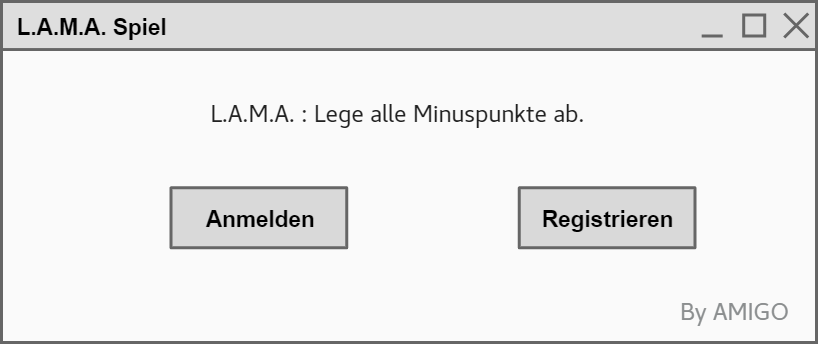
\includegraphics[width=0.7\textwidth]{img/willkommen}
	\caption{Willkommens$-$Fenster.}
	\label{gui:willkommen}
\end{figure}
\begin{figure}
	\centering
	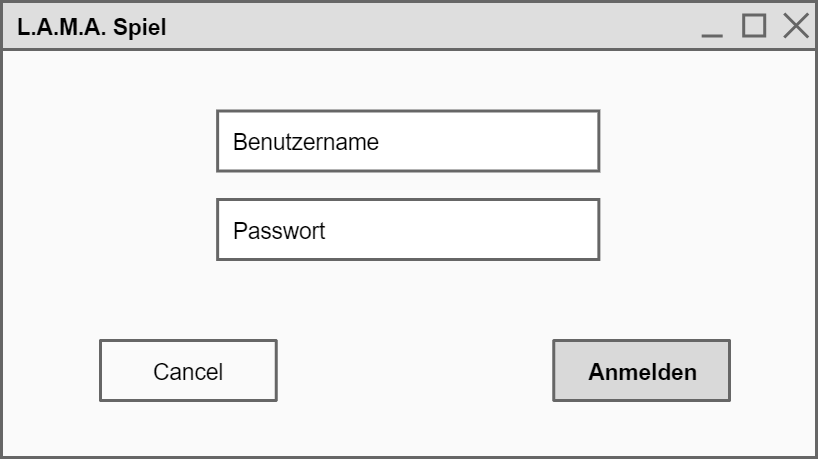
\includegraphics[width=0.7\textwidth]{img/Anmelden}
	\caption{Skizze einer GUI zum Einloggen.}
	\label{gui:login}
\end{figure}
\begin{figure}
	\centering
	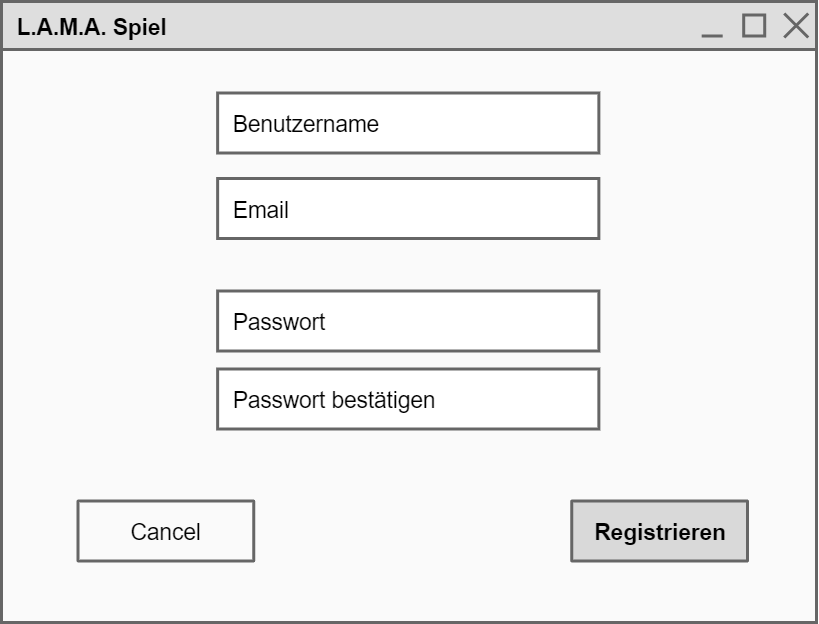
\includegraphics[width=0.7\textwidth]{img/registrieren}
	\caption{Skizze einer GUI zum Registrierung.}
	\label{gui:register}
\end{figure}
\begin{figure}
	\centering
	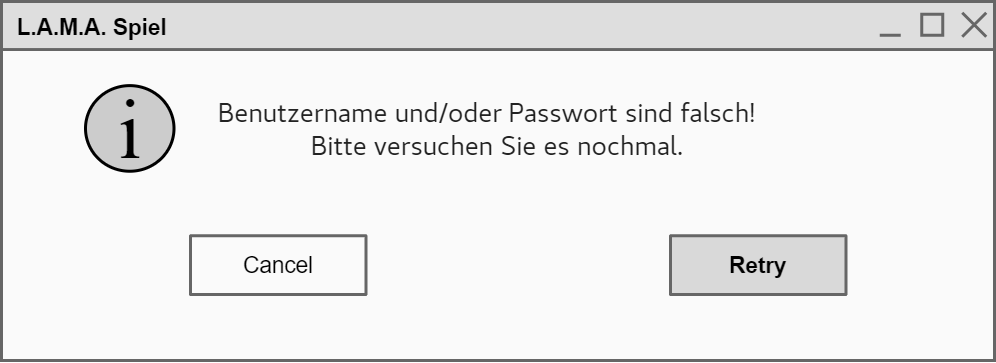
\includegraphics[width=0.7\textwidth]{img/falschername}
	\caption{Skizze einer GUI für einen Anmeldungsfehler.}
	\label{gui:warning1}
\end{figure}
\begin{figure}
	\centering
	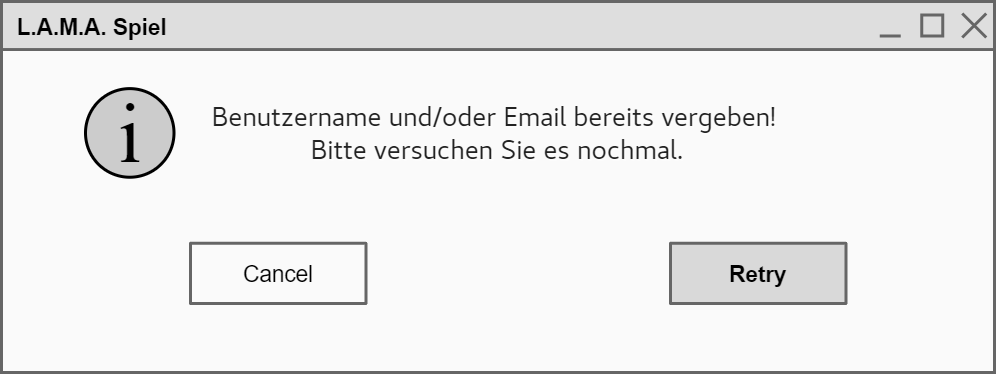
\includegraphics[width=0.6\textwidth]{img/namevergeben}
	\caption{Skizze einer GUI für einen Registrierungsfehler.}
	\label{gui:warning2}
\end{figure}
\begin{figure}
	\centering
	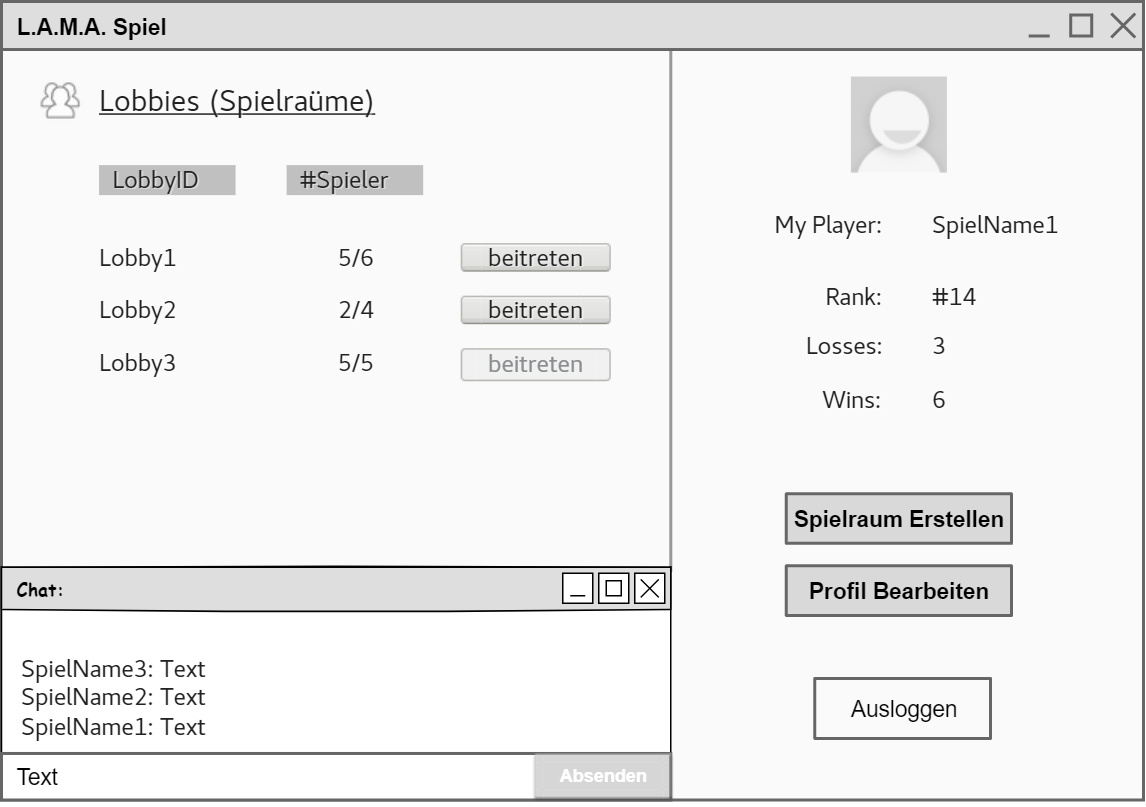
\includegraphics[width=0.7\textwidth]{img/Startseite}
	\caption{Skizze einer GUI für die Startseite.}
	\label{gui:profil}
\end{figure}
\begin{figure}
	\centering
	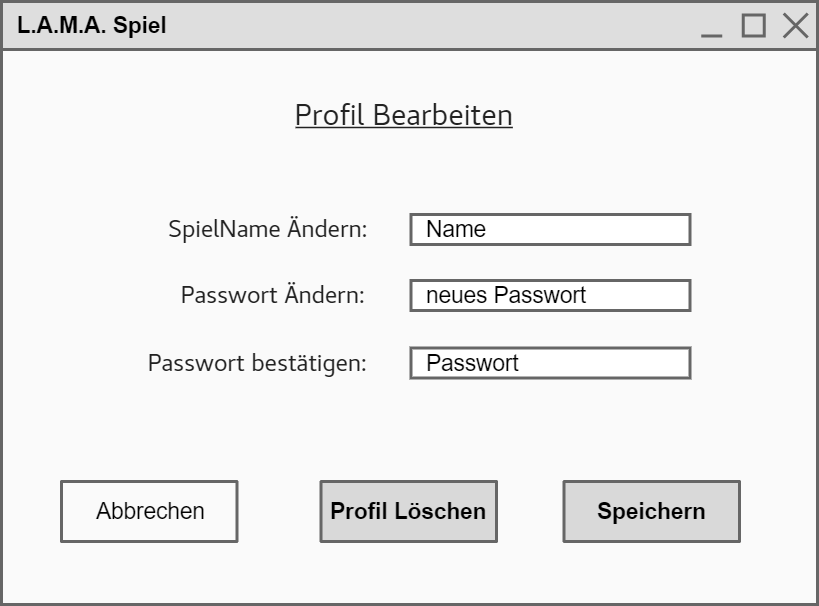
\includegraphics[width=0.7\textwidth]{img/profilbear2}
	\caption{Skizze einer GUI, um das Profil des Spielers zu bearbeiten.}
	\label{gui:modifieprofil}
\end{figure}
\begin{figure}
	\centering
	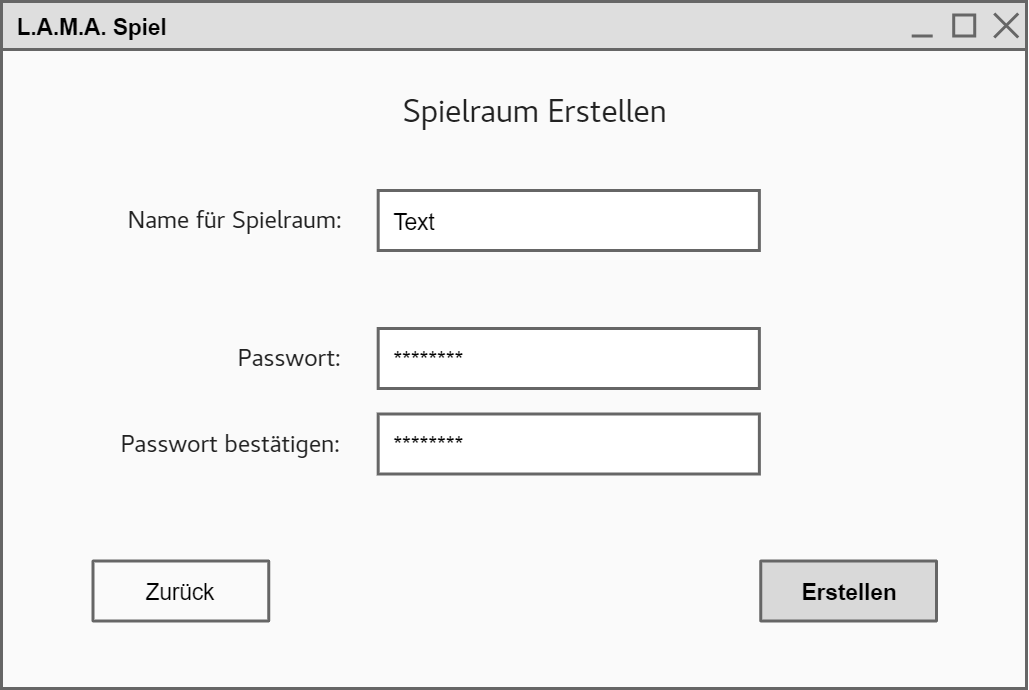
\includegraphics[width=0.7\textwidth]{img/spielraumerstellen}
	\caption{Skizze einer GUI, um eine neue Lobby(Spielraum) zu erstellen.}
	\label{gui:spielraumerstellen}
\end{figure}
\begin{figure}
	\centering
	\includegraphics[width=0.7\textwidth]{img/Lobby}
	\caption{Skizze einer GUI, wenn der Spieler einer Lobby beitritt, um das Spiel zu starten.}
	\label{gui:lobby}
\end{figure}
\begin{figure}
	\centering
	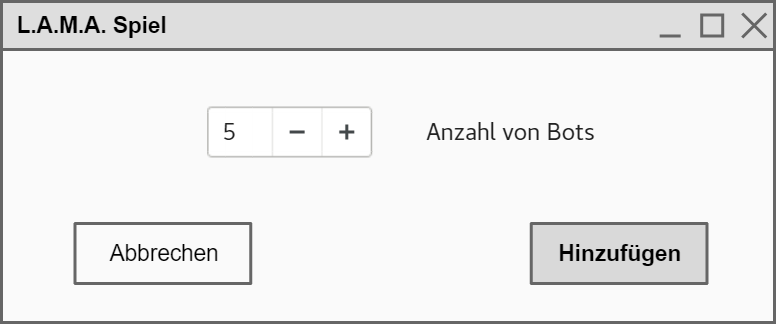
\includegraphics[width=0.7\textwidth]{img/addplayer2}
	\caption{Skizze einer GUI, um Bots in die Lobby hinzuzufügen.}
	\label{gui:addplayer}
\end{figure}
\begin{figure}
	\centering
	\includegraphics[width=0.9\textwidth]{img/spielbrett}
	\caption{Skizze einer GUI für das Spielbrett.}
	\label{gui:game}
\end{figure}
\begin{figure}
	\centering
	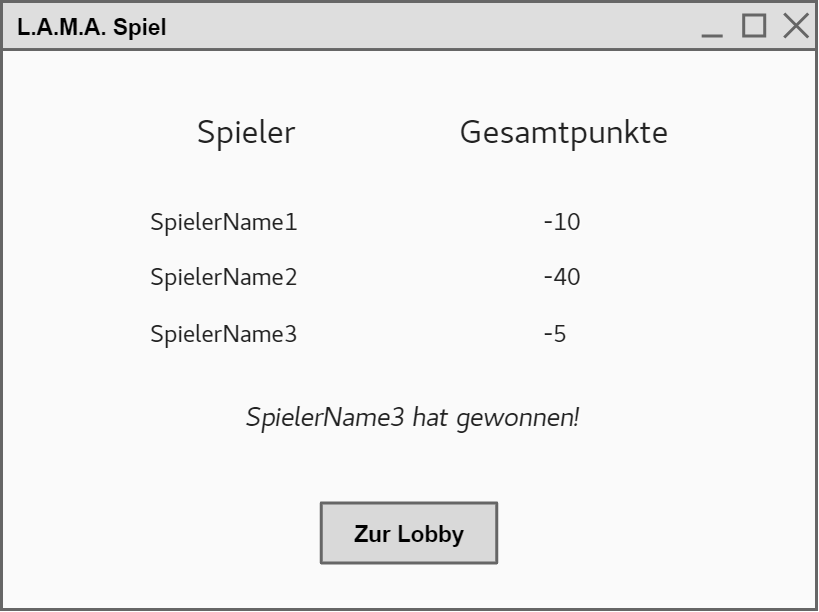
\includegraphics[width=0.7\textwidth]{img/spielbeendet}
	\caption{Skizze einer GUI für die Ergebnisse nach einem Spiel.}
	\label{gui:results}
\end{figure}
\begin{figure}
	\centering
	\includegraphics[width=0.9\textwidth]{img/alles3}
	\caption{Darstellung der Zusammenhänge zwischen GUI-Ansichten.}
	\label{gui:zusammenhang}
\end{figure}
